\documentclass{beamer}

\usepackage[utf8]{inputenc} % Language and font encoding
\usepackage[icelandic]{babel}
\usepackage[T1]{fontenc}


\usepackage{tikz}
\usepackage[listings,theorems]{tcolorbox}
\usepackage{booktabs}
\usepackage{minted} %Minted and configuration
\usemintedstyle{default}

\renewcommand{\theFancyVerbLine}{\sffamily \arabic{FancyVerbLine}}
%%%%%%%%%%%
% More math
%%%%%%%%%%%
\newcommand{\Mod}[1]{\ \text{mod}\ #1}

%%%%%%%%%%%%%%%%%%%%%%
% Beamer configuration
%%%%%%%%%%%%%%%%%%%%%%
\setbeamertemplate{navigation symbols}{}
\usecolortheme{dove}
\setbeamercolor{frametitle}{fg=white}

\usebackgroundtemplate%
{%
\vbox to \paperheight{

\includegraphics[width=\paperwidth]{Pics/hi-slide-head-2016}

\vfill
\hspace{0.5cm}
\includegraphics[width=0.3\paperwidth]{Pics/hi-von-logo}
\vspace{0.4cm}
    }%
}

\AtBeginSection[]
{
  \begin{frame}<beamer>
    \frametitle{Yfirlit}
    \tableofcontents[currentsection]
  \end{frame}
}

\setbeamerfont{frametitle}{size=\normalsize}
\addtobeamertemplate{frametitle}{}{\vspace*{0.5cm}}

%%%%%%%%%%%%%%%%%%%%%%%%%
% tcolorbox configuration
%%%%%%%%%%%%%%%%%%%%%%%%%

% Setup from: http://tex.stackexchange.com/a/43329/21638
\tcbset{%
    noparskip,
    colback=gray!10, %background color of the box
    colframe=gray!40, %color of frame and title background
    coltext=black, %color of body text
    coltitle=black, %color of title text 
    fonttitle=\bfseries,
    alerted/.style={coltitle=red, colframe=gray!40},
    example/.style={coltitle=black, colframe=green!20, colback=green!5},
}


%%%%%%%%%%%%%%%%%%%%%%%
% Further configuration
%%%%%%%%%%%%%%%%%%%%%%%
\hypersetup{colorlinks=true,pdfauthor={Eirikur Ernir Thorsteinsson},linkcolor=blue,urlcolor=blue}
\graphicspath{{./Pics/}}

\author{Eiríkur Ernir Þorsteinsson}
\institute{Háskóli Íslands}
\date{Haust 2016}

\title{Tölvunarfræði 1a}
\subtitle{Vika 13, seinni fyrirlestur}

\begin{document}

\begin{frame}
\titlepage
\end{frame}

\section{Inngangur}

\begin{frame}{Í síðasta þætti\ldots}
\begin{itemize}
 \item Tölfræði
 \item Mengi
\end{itemize}
\end{frame}

\section{Margliður}

\begin{frame}[fragile]{Margliður}
\begin{itemize}
 \item Margliður þarf ekki að kynna, þær eru jöfnur á forminu
\[
 a_0x^n + a_1x^{n-1} + \ldots a_nx^0
\]
 \item Matlab getur unnið með margliður
 \item Þær eru táknaðar sem línuvigur af tölum sem tákna stuðla margliðunnar
 \begin{itemize}
  \item Margliðan $x^3 + 2x^2 -4x +3$ væri þá táknuð með vigrinum \verb|[1 2 -4 3]|
 \end{itemize} 
\end{itemize}
\end{frame}

\begin{frame}[fragile]{Að vinna með margliður}
\begin{columns}
\column{0.6\textwidth}
Dæmi um fall sem unnið getur með margliður er fallið \texttt{roots}. Reiknum rætur margliðunnar $3x^2 + 2x - 2$:
\begin{minted}[frame=lines]{matlab}
>> p = [3 2 -2];
>> roots(p)
ans =
   -1.2153
    0.5486
\end{minted}
\column{0.4\textwidth}
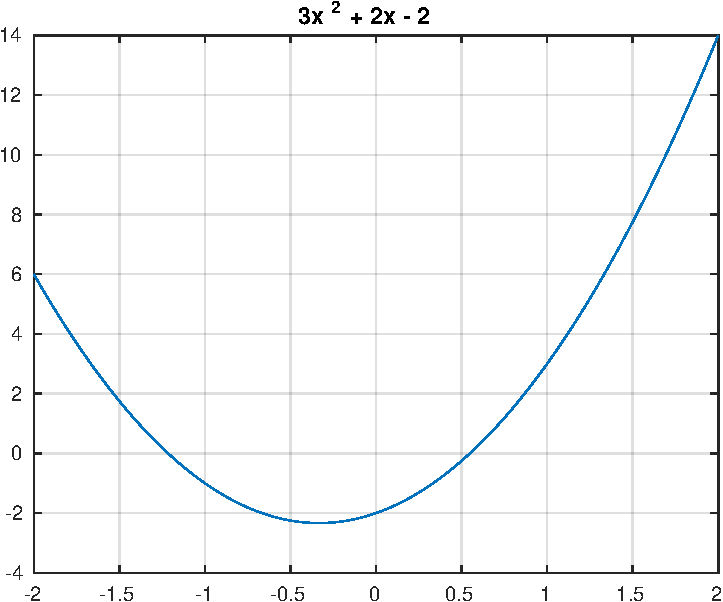
\includegraphics[width=\linewidth]{Pics/poly-example}
\end{columns}
\end{frame}

\begin{frame}[fragile]{Að vinna með margliður}
Hægt er að meta gildi margliðu í ákveðnum punkti með fallinu \texttt{polyval}.
\begin{minted}[frame=lines]{matlab}
>> p = [3 2 -2];
>> polyval(p,0)
ans =
    -2
>> polyval(p,2)
ans =
    14
\end{minted}
\end{frame}

\section{Nálgun og brúun (14.1.2-3)}

\begin{frame}{Punktar og ferlar}
\begin{itemize}
 \item Höfum $n$ punkta með gildum $(x_1,y_1),(x_2,y_2),\ldots,(x_n,y_n)$
 \item Algeng vandamál:
 \begin{itemize}
  \item Þurfum að finna feril sem ``líkist'' gagnapunktunum
  \begin{itemize}
   \item Ákveðum að punktarnir séu á t.d. línu eða fleygboga
   \item Kallast nálgun ferils (e. \emph{curve fitting}) 
  \end{itemize}
  \item Þurfum fleiri gagnapunkta
  \begin{itemize}
   \item Áætlum $y$-gildi fyrir $x$ sem er á milli $x_i$ og $x_{i+1}$ eða gildi sem er utan sviðs $x$
   \item Kallast brúun (e. \emph{interpolation}) eða framreikningur (e. \emph{extrapolation})
  \end{itemize}
 \end{itemize}
\end{itemize}
\end{frame}

\subsection{Nálgun punkta}

\begin{frame}[fragile]{Dæmi}
\begin{columns}
\small
\column{0.6\textwidth}
\begin{itemize}
 \item Höfum gögn um vindhraða á 3ja tíma fresti í Skaftafelli 
 \begin{itemize}
  \item klukkan 3:00 er vindhraðinn 15.2 m/s, klukkan 6:00 er hann 17.7 m/s, o.s.frv.
 \end{itemize}
 \item Hvaða ferill passar best við þessi gildi?
 \item Hver var vindhraðinn klukkan 14:00?
\end{itemize}
\column{0.4\textwidth}
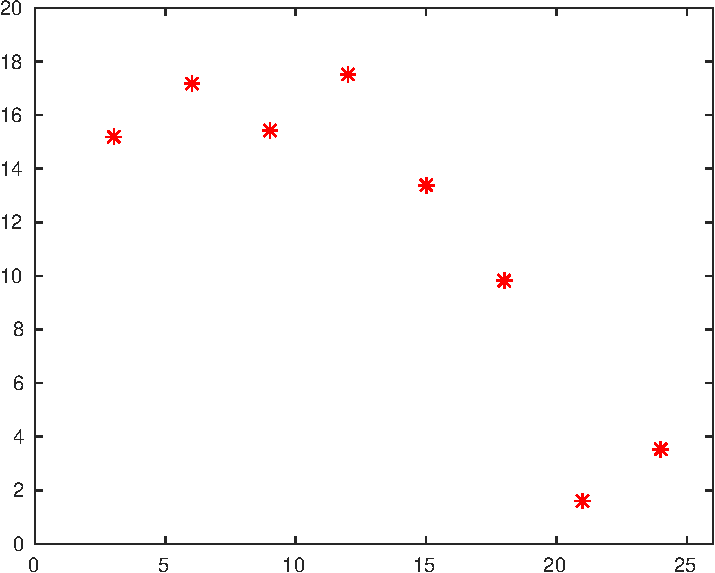
\includegraphics[width=\linewidth]{Pics/vindur}
\end{columns}
\begin{minted}[fontsize=\small]{matlab}
>> wind = [15.2 17.2 15.4 17.5 13.4 9.8 1.6 3.5];
>> time = 3:3:24;
>> plot(time, wind, 'r*'); 
>> axis([0 26 0 20])
\end{minted}
\end{frame}

\begin{frame}[fragile]{Að finna bestu margliðu}
\begin{itemize}
 \item Vindgögnin eru dæmi um ``tilraunagögn'' sem við gætum viljað máta við ýmsar gerðir margliða
 \begin{itemize}
  \item Finna bestu línu, besta fleygboga, bestu þriðja stigs margliðu, o.s.frv.
 \end{itemize}
 \item Fallið \texttt{polyfit} finnur bestu margliðu fyrir gögnin samkvæmt aðferð minnstu fervika (e. \emph{least squares method})
\begin{minted}{matlab}
p = polyfit(x, y, degree)
\end{minted}
\begin{itemize}
 \item Þar sem \texttt{p} er besta margliðan, \texttt{x} og \texttt{y} eru vigrar af gögnum, og \texttt{degree} er stig margliðunnar sem mynda skal
\end{itemize}
\end{itemize}
\end{frame}

\begin{frame}[fragile]{Besta lína fyrir vindgögnin}
\vspace{\baselineskip}
Notum \texttt{polyfit} og \texttt{polyval} saman til að teikna bestu línu
\begin{minted}[frame=lines, fontsize=\small]{matlab}
>> wind = [15.2 17.2 15.4 17.5 13.4 9.8 1.6 3.5];
>> time = 3:3:24;
>> plot(time, wind, 'r*');
>> axis([0 26 0 20])
>> lineEquation = polyfit(time, wind, 1)
lineEquation =
   -0.7175   21.3857
>> line = polyval(lineEquation, time);
>> hold on
>> plot(time, line)
\end{minted}
Hér reyndist besta línan vera $y = -0.7175x + 21.3857$
\end{frame}

\begin{frame}[fragile]{Besti fleygbogi fyrir vindgögnin}
\begin{minted}[frame=lines, fontsize=\small]{matlab}
>> parabolicEquation = polyfit(time, wind, 2);
>> xi = linspace(min(time),max(time));
>> parabola = polyval(parabolicEquation, x);
>> plot(time, wind, 'r*', xi, parabola, 'b-')
>> axis([0 26 0 20])
\end{minted}
\begin{columns}
\column{0.5\textwidth}
\small
Athugum: Þurfum hærri upplausn á fleygboganum til að myndin komi vel út

Trix: Plot getur teiknað marga ferla í einu
\column{0.5\textwidth}
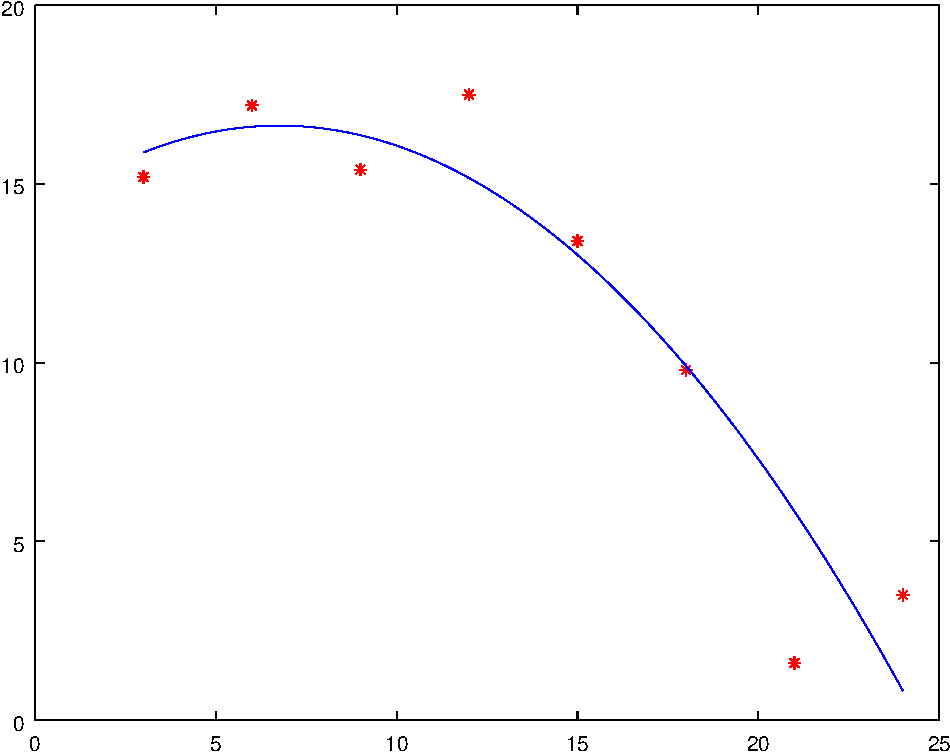
\includegraphics[width=\linewidth]{Pics/wind-parabola}
\end{columns}
\end{frame}

\begin{frame}[fragile]{Bestu margliður}
\begin{minted}[frame=lines, fontsize=\small]{matlab}
wind = [15.2 17.7 15.4 17.5 13.4 9.8 1.6 3.5];
time = 3:3:24;
xi = linspace(min(time),max(time));
for degree = 1:3
   coefficients = polyfit(time, wind, degree);
   curve = polyval(coefficients, xi);
   subplot(1, 3, degree)
   plot(time, wind, 'r*', xi, curve)
   xlabel('Tími')
   ylabel('Vindhraði')
   title(sprintf('%d. stigs margliða', degree))
   axis([0 26 0 20]);
end
\end{minted}
\end{frame}

\begin{frame}[fragile]{Bestu margliður}
\begin{center}
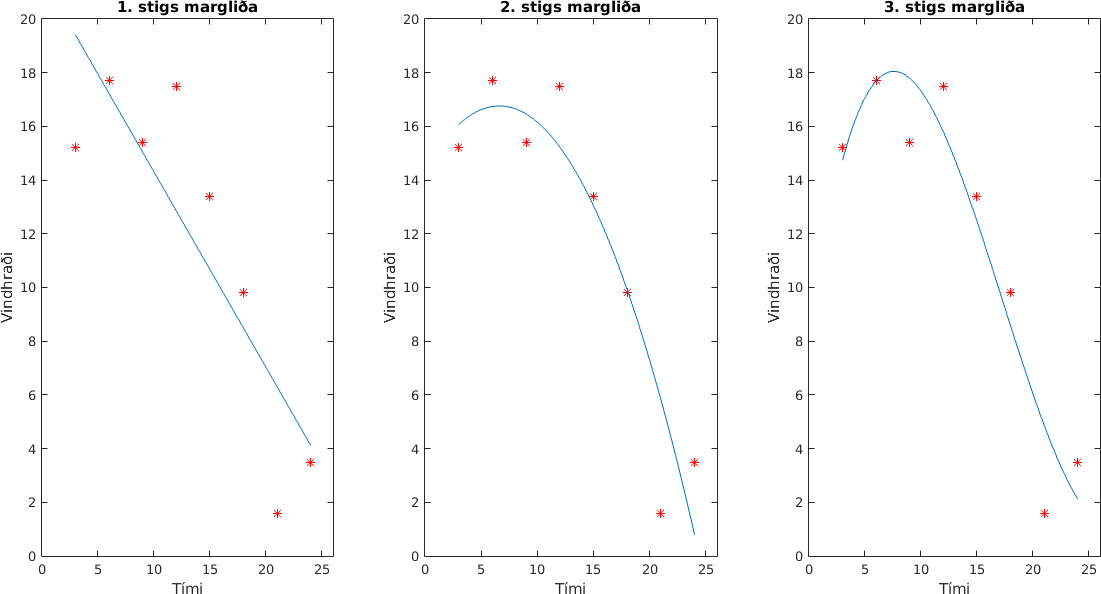
\includegraphics[height=0.6\textheight]{Pics/poly-subplot}
\end{center}
\end{frame}


\subsection{Brúun punkta}

\begin{frame}[fragile]{Brúun punkta}
\begin{itemize}
 \item Brúunarferlar verða að fara í gegnum gagnapunktana
 \item Brúað er með bútum af ferlum, bútarnir eru oft ferlar margliða
 \begin{itemize}
  \item Línuleg brúun: línur á milli gagnapunkta
  \item Annars stigs brúun:  fleygbogi á milli hverra þriggja punkta
  \item Þriðja stigs brúun (cubic):  þriðja stigs margliða á milli hverra fjögurra punkta
  \item Splæsibrúun (spline): margliða af lágu stigi með samfellda 2. afleiðu á bútaskilum
  \begin{itemize}
   \item Ferillinn verður ``mjúkur''
   \item Oft 3. stigs margliður
  \end{itemize}
 \end{itemize}
\end{itemize}
\end{frame}

\begin{frame}[fragile]{Fallið \texttt{interp1}}
Matlab-fallið \texttt{interp1} brúar vigra
\begin{center}
\texttt{yi = interp1(x, y, xi, aðferð);}
\end{center}
Hér er \texttt{yi} gildi brúunar í punktunum \texttt{xi}, \texttt{x} og \texttt{y} eru gagnapunktar, \texttt{xi} eru \texttt{x}-gildin í hærri upplausn og ``aðferð'' er t.d.  \texttt{'linear'}, \texttt{'pchip'} (cubic) eða \texttt{'spline'}.
\end{frame}

\begin{frame}[fragile]{Fallið \texttt{interp1}}
\vspace{1cm}
\begin{minted}[frame=lines, fontsize=\small]{matlab}
>> xi = linspace(min(time),max(time));
>> yi = interp1(time, wind, xi, 'pchip');
>> plot(time, wind, 'r*', xi, yi)
\end{minted}
\begin{columns}
\column{0.5\textwidth}
3. stigs brúun fyrir vindgögnin.
\column{0.5\textwidth}
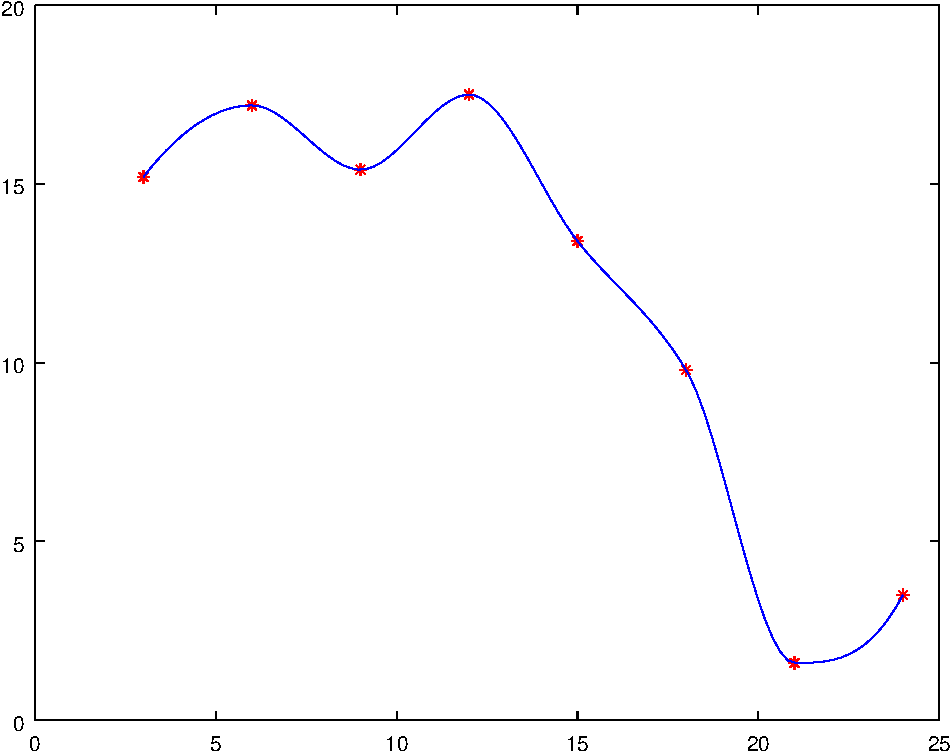
\includegraphics[width=\linewidth]{Pics/interp1-plot}
\end{columns}
\end{frame}

\begin{frame}[fragile]{Fallið \texttt{interp2}}
\begin{minted}[frame=lines, fontsize=\small]{matlab}
>> x = 1:4; y=1:4;
>> z = randi([5,10], 4, 4);
>> [xi, yi] = meshgrid(1:0.1:4, 1:0.1:4);
>> zi = interp2(x,y,z,xi,yi,'spline');
>> surf(xi,yi,zi);
\end{minted}
\begin{columns}
\column{0.5\textwidth}
Matlab hefur líka fallið \texttt{interp2}, sem brúar tvívíð gögn.
\column{0.5\textwidth}
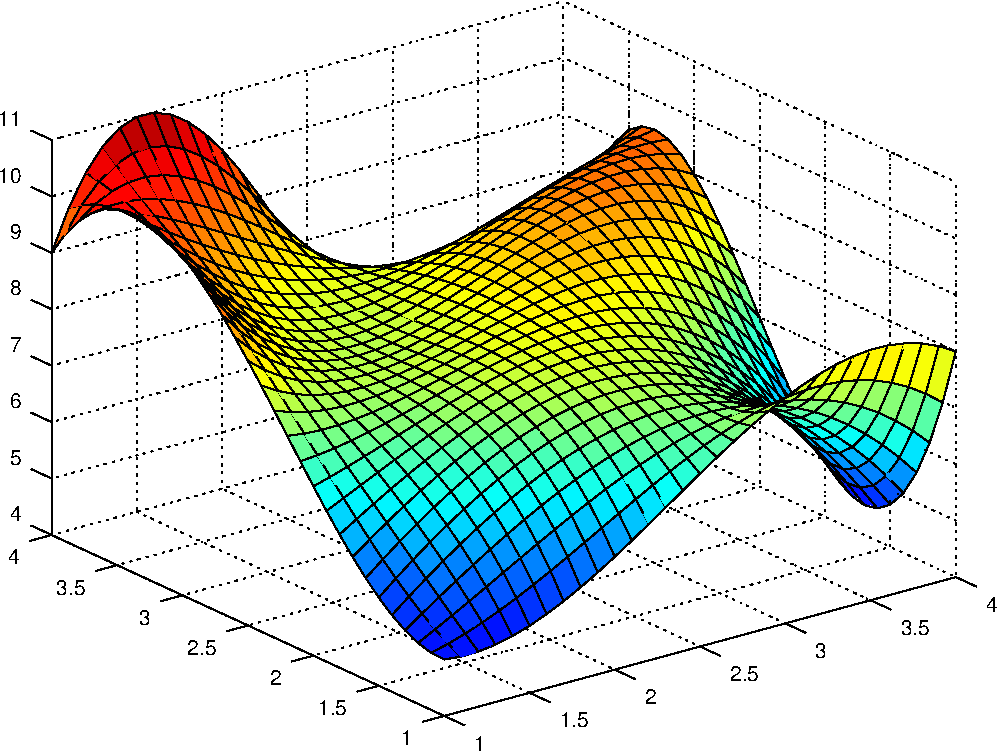
\includegraphics[width=\linewidth]{Pics/interp2-surf}
\end{columns}
\end{frame}


\begin{frame}{Fyrirlestraræfing}
\begin{columns}
\column{0.3\textwidth}
\scriptsize
\begin{tabular}{ll}
\toprule
Ár&Fjöldi\\
\midrule
2000&279.049\\
2001&283.361\\
2002&286.575\\
2003&288.471\\
2004&290.570\\
2005&293.577\\
2006&299.891\\
2007&307.672\\
2008&315.459\\
2009&319.368\\
2010&317.630\\
2011&318.452\\
2012&319.575\\
2013&321.857\\
2014&325.671\\
2015&329.100\\
\bottomrule
\end{tabular}

\column{0.7\textwidth}
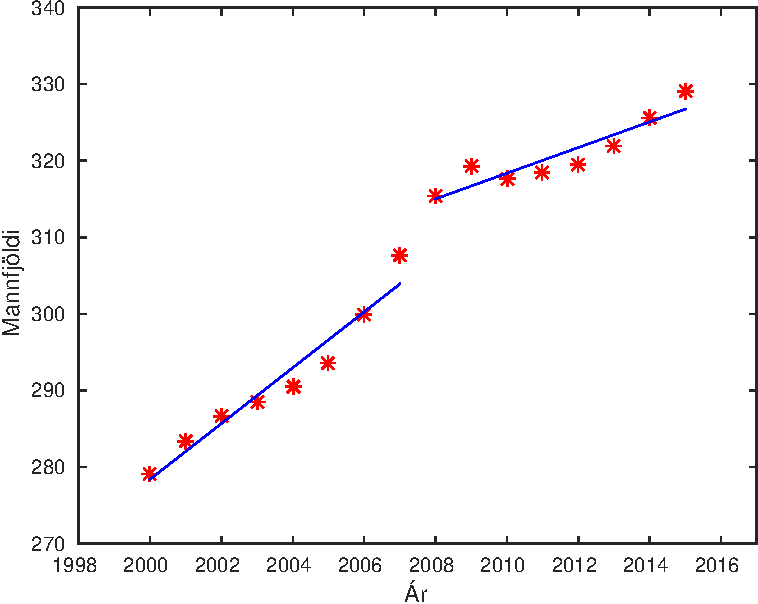
\includegraphics[width=\linewidth]{Pics/kreppa}
\end{columns}
\end{frame}
\end{document}
